\documentclass[12pt]{article}
 \usepackage[margin=1in]{geometry}
 \usepackage{amsmath,amsthm,mathtools, amssymb,amsfonts,listings,color,graphicx,titlesec,lipsum,pdfpages}

\newcommand{\N}{\mathbb{N}}
\newcommand{\Z}{\mathbb{Z}}
\newcommand{\R}{\mathbb{R}}
\newcommand{\E}{\mathbb{E}}
\newcommand{\V}{\mathbb{V}}
\newcommand{\X}{\mathbf{X}}
\newcommand{\qsum}{\sum\limits_{i=1}^n}
\newcommand{\vpar}{\vspace{.3cm}}

\begin{document}
\title{Econ 675: HW 4}
\author{Erin Markiewitz}
\maketitle
\newpage
\tableofcontents
\newpage

\section{Estimating Equations}
This question considers identification under selection-on-observables for the generaic class of parameters
\begin{align*}
\theta_t(g) = \E[g(Y_i(t))], \ g \in G, \ t \in T
\end{align*}

where $G$ denotes a class of functions (e.g. $G = \{ \mathbf{1}(. \leq y) : y \in \R)\}$). Define the regression functions:
\begin{align*}
  p_t(\mathbf{X_i} = \P[T_i = t| \\
  \mathbf{X_i}]), e_t(g;\mathbf{X_i}) = \E[g(Y_i(t))|\mathbf{X_i}] = = \E[g(Y_i(t))|\mathbf{X_i}, T_i =1], \ g \in G, \ t \in T
\end{align*}

Assume Ignorability: $Y_i(t) \bot D_i(t) |\mathbf{X_i}$ and $0 < x < p_t(\X_i)$, for all $t \in T$ and for some fixed positive constant c.
\subsection{}
In the following section, we prove the validity of three moment cofitions for the generic class of parameters. The first moment condition is the Inverse Probabiltiy Weighting (IPW) moment condition.

\begin{align*}
\psi_{IPW,t}(\mathbf{Z}_i;\theta_t(g)) = \frac{D_i(t)\cdot g(Y_i(t))}{p_t(\X_i)} - \theta_t(g)
\end{align*}

To begin, take the expectation of the moment condition.

\begin{align*}
\E\left[\frac{D_i(t)\cdot g(Y_i(t))}{p_t(\X_i)}\right] - \theta_t(g)
\end{align*}

By the law of iterative expectations
\begin{align*}
  \E\left[\E\left[\frac{D_i(t) \cdot g(Y_i(t))}{p_t(\X_i)} |\X_i \right] \right] - \theta_t(g)
\end{align*}

\begin{align*}
  \E\left[\frac{1}{p_t(\X_i)}  \E\left[D_i(t) \cdot g(Y_i(t)) |\X_i \right] \right] - \theta_t(g)
\end{align*}

\begin{align*}
  \E\left[\frac{1}{p_t(\X_i)}  \E\left[D_i(t)|\X_i \right] \cdot \E\left[g(Y_i(t)) |\X_i \right] \right] - \theta_t(g)
\end{align*}


As $\E\left[D_i(t)|\X_i \right] = \Pr \left[D_i(t) = 1|\X_i \right] = \Pr \left[T_i= t|\X_i \right] =p_t(\X_i)$

\begin{align*}
  \E\left[\frac{p_t(\X_i)}{p_t(\X_i)} \cdot \E\left[g(Y_i(t)) |\X_i \right] \right] - \theta_t(g)
\end{align*}

which gives us our result,

\begin{align*}
  \E\left[\E\left[g(Y_i(t)) |\X_i \right]\right] - \theta_t(g) = \E\left[g(Y_i(t))\right] - \theta_t(g) = \theta_t(g) -\theta_t(g) = 0
\end{align*}


The second moment condition of this exercise is the Regression Imputation (1) moment condition:

\begin{align*}
\psi_{RI1,t}(\mathbf{Z}_i;\theta_t(g)) =  e_t(g;\X_i)- \theta_t(g)
\end{align*}

Take the expectation

\begin{align*}
\E\left[ e_t(g;\X_i)  \right]  - \theta_t(g)
\end{align*}

\begin{align*}
\E\left[\E\left[ g(Y_i(t)) | \X_i \right]  \right]  - \theta_t(g)
\end{align*}

\begin{align*}
\E\left[g(Y_i(t)) \right] - \theta_t(g) = \theta_t(g) -\theta_t(g) =0
\end{align*}

The second moment condition of this exercise is the Regression Imputation (2) moment condition, which includes inverse probabilty weighting:

\begin{align*}
\psi_{RI2,t}(\mathbf{Z}_i;\theta_t(g)) =  \frac{D_i(t) \cdot e_t(g;\X_i)}{p_t(\X_i)}- \theta_t(g)
\end{align*}

Take the expectation

\begin{align*}
\E \left[ \frac{D_i(t) \cdot e_t(g;\X_i)}{p_t(\X_i)}\right]  - \theta_t(g)
\end{align*}

iterate the expectation a bit

\begin{align*}
\E \left[ \frac{1}{p_t(\X_i)} p_t(\X_i) \cdot \E\left[ g(Y_i(t)) | \X_i \right] \right]  - \theta_t(g)
\end{align*}

which gives the result

\begin{align*}
\E\left[g(Y_i(t)) \right] - \theta_t(g) = \theta_t(g) -\theta_t(g) =0
\end{align*}

Last, we consider the doubly robust estimator's moment condition:

\begin{align*}
\psi_{DR,t}(\mathbf{Z}_i;\theta_t(g)) =  \frac{D_i(t) \cdot g(Y_i(t))}{p_t(\X_i)}- \theta_t(g) -  \frac{e_t(g;\X_i)}{p_t(\X_i)} \cdot (D_i(t) -  p_t(\X_i))
\end{align*}

Take expectations

\begin{align*}
 \E \left[\frac{D_i(t) \cdot g(Y_i(t))}{p_t(\X_i)} \right] - \theta_t(g) -  \E\left[\frac{e_t(g;\X_i)}{p_t(\X_i)} \cdot (D_i(t) -  p_t(\X_i))\right]
\end{align*}

From previous results the first two terms cancel,

\begin{align*}
- \E\left[\frac{D_i(t)\cdot e_t(g;\X_i) }{p_t(\X_i)} \right]  + \E \left[  e_t(g;\X_i) \right]
\end{align*}

The result follows from the law of iterated expectations.

\subsection{}
The IPW plug-in estimator:

\begin{align*}
\hat\psi_{IPW,t}(\mathbf{Z}_i;\theta_t(g)) = \frac{1}{n}\qsum\frac{D_i(t) \cdot g(Y_i) }{\hat p_t(\X_i)}
\end{align*}

Where $\hat p_t(\X_i)$ is the estimated propensity score from the first-stage regression of the treatment on the covariates.

To write down the RI1 plug-in estimator, start by putting a hat on it:

\begin{align*}
\hat\psi_{RI1,t}(\mathbf{Z}_i) =\frac{1}{n}\qsum \hat e_t(\X_i)
\end{align*}

where $\hat e_t(X_i) = \E[g(Y_i(t))|\X_i, T_i =t]$, the conditional expectation of the class of regression functions specified by $G$. We can rewrite the estimator above as:

\begin{align*}
\hat\psi_{RI1,t}(\mathbf{Z}_i) = \frac{1}{n}\qsum\frac{D_i(t) \cdot \hat e_t(\X_i)}{\hat p_t(\X_i)}
\end{align*}

To write down the RI1 plug-in estimator, just reweight using the estimated propensity score:

\begin{align*}
\hat\psi_{RI2,t}(\mathbf{Z}_i) = \frac{1}{n}\qsum\frac{D_i(t) \cdot \hat e_t(\X_i)}{\hat p_t(\X_i)}
\end{align*}

And the double robust plug in estimator

\begin{align*}
\hat\psi_{DR,t}(\mathbf{Z}_i) = \frac{1}{n}\qsum\frac{D_i(t) \cdot g(Y_i)}{\hat p_t(\X_i)}
-\frac{1}{n}\qsum\frac{\hat e_t(\X_i)}{\hat p_t(\X_i)} (D_i(t) - \hat p_t(\X_i))
\end{align*}

The relative performance of the estimators depends on the data generating process.
As the IPW and R2 plug in estimators use the estimated propensity score reweight the treatment effects, both estimators will be inconsistent in finite samples when the propensity score is very close to either one or zero. (If you are only estimating the treatement effect on the treated, it is sufficient that the propensity score is not degenerative with respect to 1.) The double robust estimators includes further safeguards against bias induced by misspecification but at the cost of imposing additional specification choices.

Then again, transparency is a key feature of an estimator - especially in policy analysis. Conditioning on covariates allow for specification of the propensity score without prior knowledge of the outcome variable/equation.

\subsection{}
(Just a hunch)
The estimating equations in section 1.1 can be used to estimate the variance of the potential outcome variables. First, we specify the function

\begin{align*}
  g(x)= (x - \E[x])^2, \ x \in \R
\end{align*}

and its finite sample analogue

\begin{align*}
  \hat g(x)= \frac{1}{n}\qsum(x_i - \frac{1}{n}\qsum x_i)^2 , \ x_i \in \X \in \R^n
\end{align*}

The validity of these moment conditions is established in section 1.1 more generally.
Under this specification of $g$, $\theta_t(g) = \V[Y_i(t)]$ and $e_t(g;\X_i) = \V[Y_i(t)|\X_i]$, the unconditional and conditional variance of the potential outcome of treatement t, respectively. This gives us the moment conditions:

\begin{align*}
\psi_{IPW,t}(\mathbf{Z}_i;\sigma_t^2) = \frac{D_i(t)\cdot   (Y_i(t) - \E[Y_i(t)])^2 }{p_t(\X_i)} - \sigma_t^2
\end{align*}

\begin{align*}
\psi_{RI1,t}(\mathbf{Z}_i;\sigma_t^2) =  \E[(Y_i(t) - \E[Y_i(t)])^2 | \X_i] - \sigma_t^2
\end{align*}

\begin{align*}
\psi_{RI2,t}(\mathbf{Z}_i;\sigma_t^2) =  \frac{D_i(t) \cdot \E[(Y_i(t) - \E[Y_i(t)])^2 | \X_i]}{p_t(\X_i)}- \sigma_t^2
\end{align*}

\begin{align*}
\psi_{DR,t}(\mathbf{Z}_i;\sigma_t^2) =  \frac{D_i(t) \cdot (Y_i(t) - \E[Y_i(t)])^2}{p_t(\X_i)}- \sigma_t^2-  \frac{\E[(Y_i(t) - \E[Y_i(t)])^2 | \X_i]}{p_t(\X_i)} \cdot (D_i(t) -  p_t(\X_i))
\end{align*}


Now in order to conduct the hypothesis test of $\mathbf{H}_0 : \sigma^2_t = \sigma^2$ we need to use the finite sample analogue of the $g$ function specified above. The variance of our moment conditions will be estimated using a simple GMM procedure. In this case, we use a two step procedure for the moment conditions that use IPW. In the first step, we estimate the propensity score and drop any observations with propensity scores sufficiently close to zero or one. For a given moment condition $M \in \{IPW,RI1,RI2,DR \} $  and treatment t we define the finite sample analogue as $\hat\psi_{M,t}$

So GMM is

\begin{align*}
  \hat{\mathbf{\Omega}}_{M,t}  = \frac{1}{n} \qsum \hat \psi_{M,t} \hat\psi_{M,t}'
\end{align*}

From Theorem 12.7.1 in Hansens's Econometrics text,

\begin{align*}
  \mathbf{\hat{V}}_{\psi,M,t} = (\hat \psi_{M,t} \hat{\mathbf{\Omega}}_{M,t}^{-1}   \hat\psi_{M,t}')^{-1}
\end{align*}

And so in order to conduct the hypothesis test we simply reject the null if $\hat\sigma_t^2$ is outside of the following confidence interval:

\begin{align*}
\mathbf{CI}_{\alpha} (\hat\sigma_t^2) = \left[\sigma^2  - \mathbf{\Phi}^{-1}(\frac{\alpha}{2}) \sqrt{\frac{\mathbf{\hat{V}}_{\psi,M,t}}{n}}   , \sigma^2  + \mathbf{\Phi}^{-1}(\frac{\alpha}{2}) \sqrt{\frac{\mathbf{\hat{V}}_{\psi,M,t}}{n}}  \right]
\end{align*}



\section{}
\section{}
\subsection{}


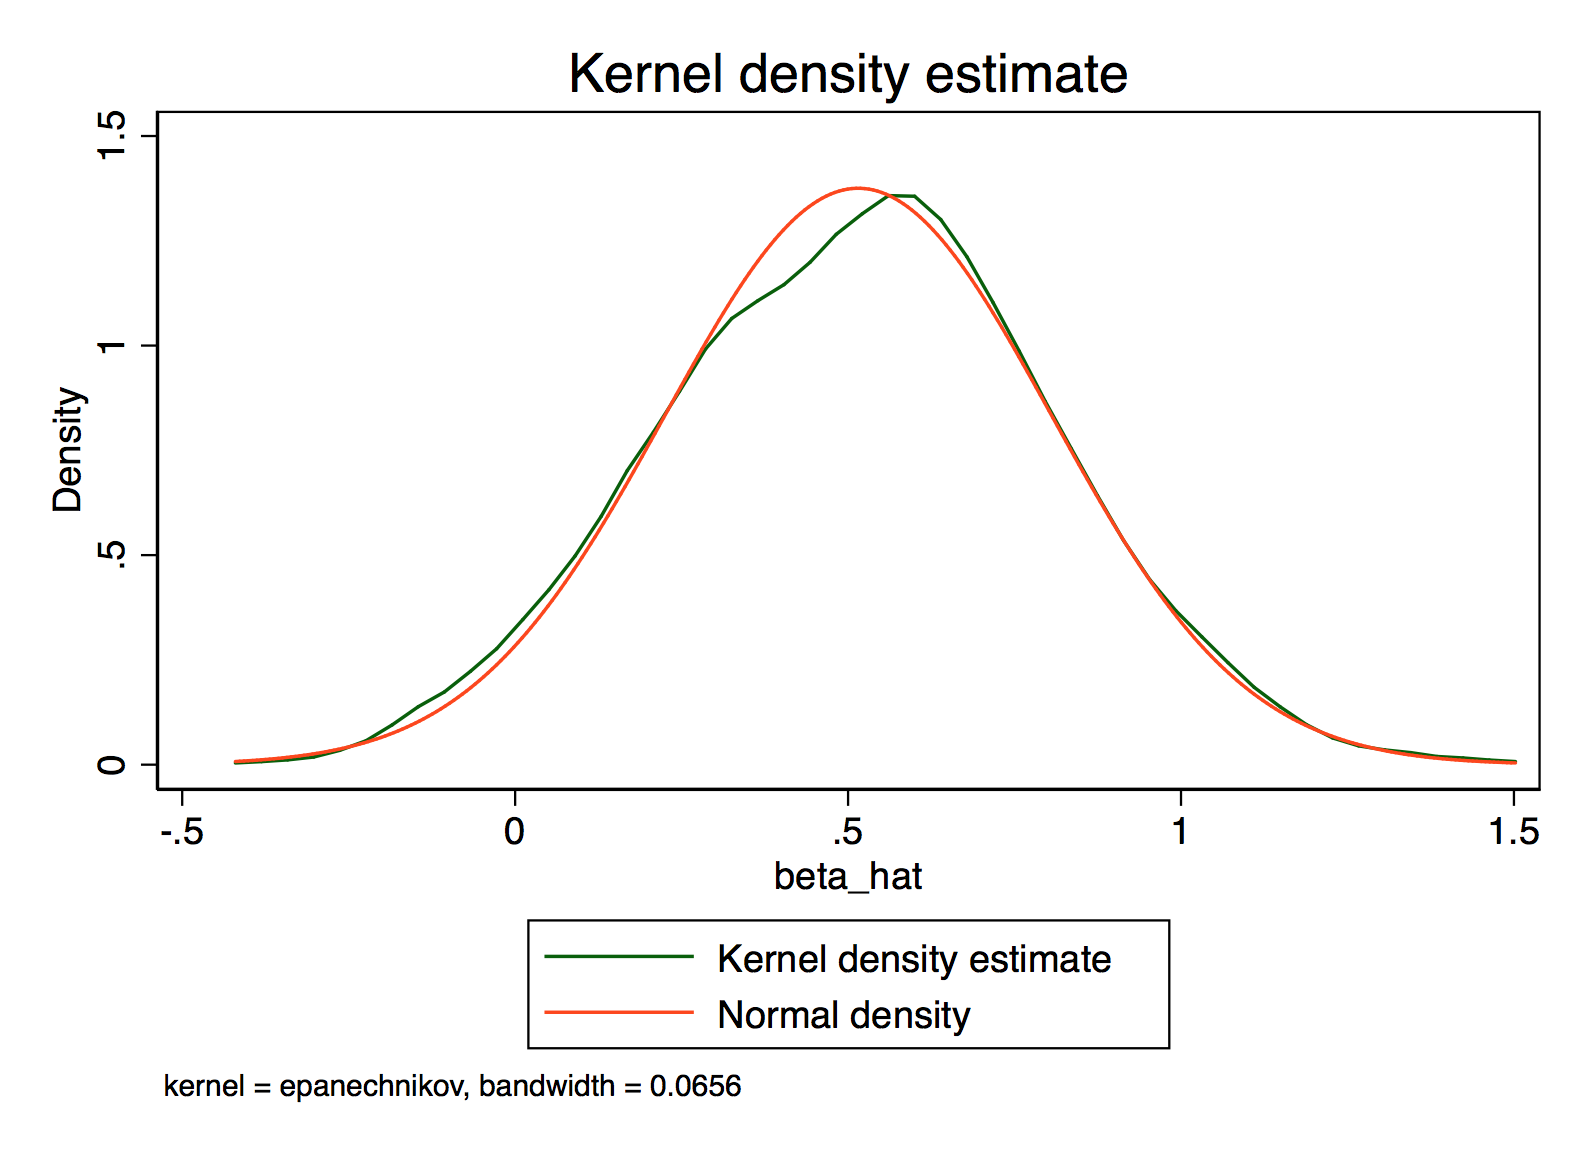
\includegraphics[totalheight=5cm]{hw4_q3_bhat_stata.png}
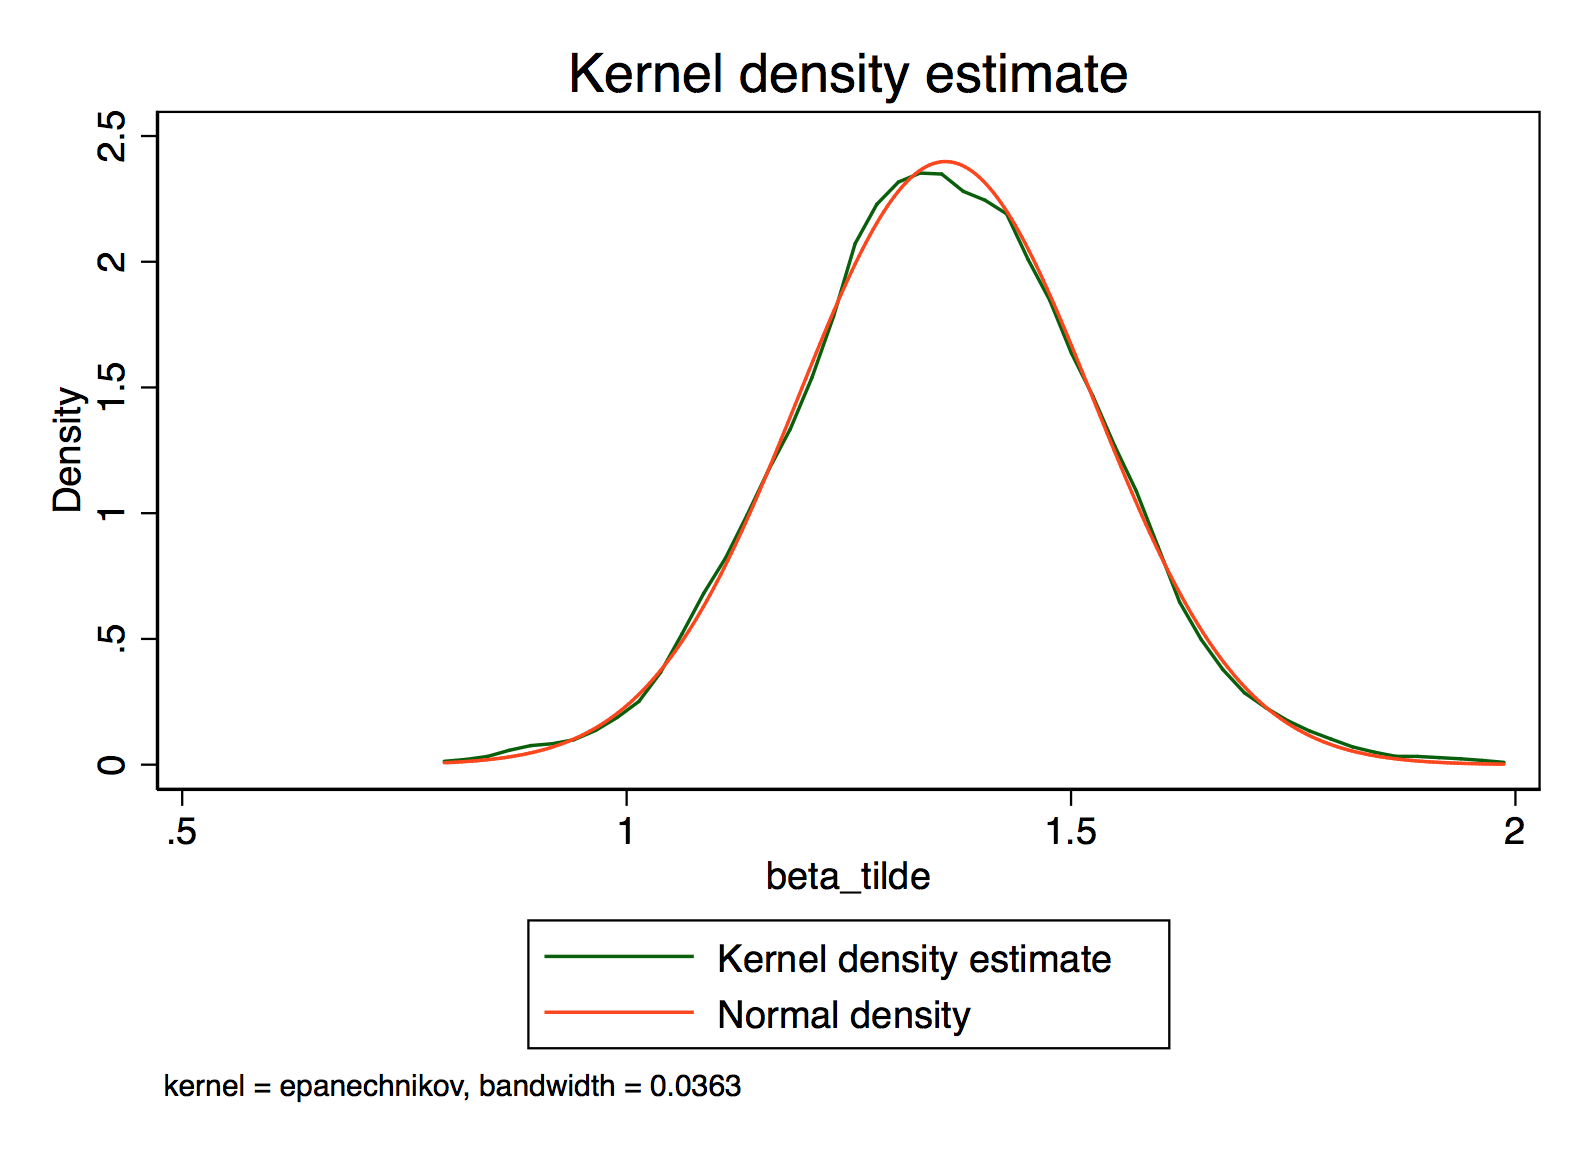
\includegraphics[totalheight=5cm]{hw4_q3_btilde_stata.png}\\
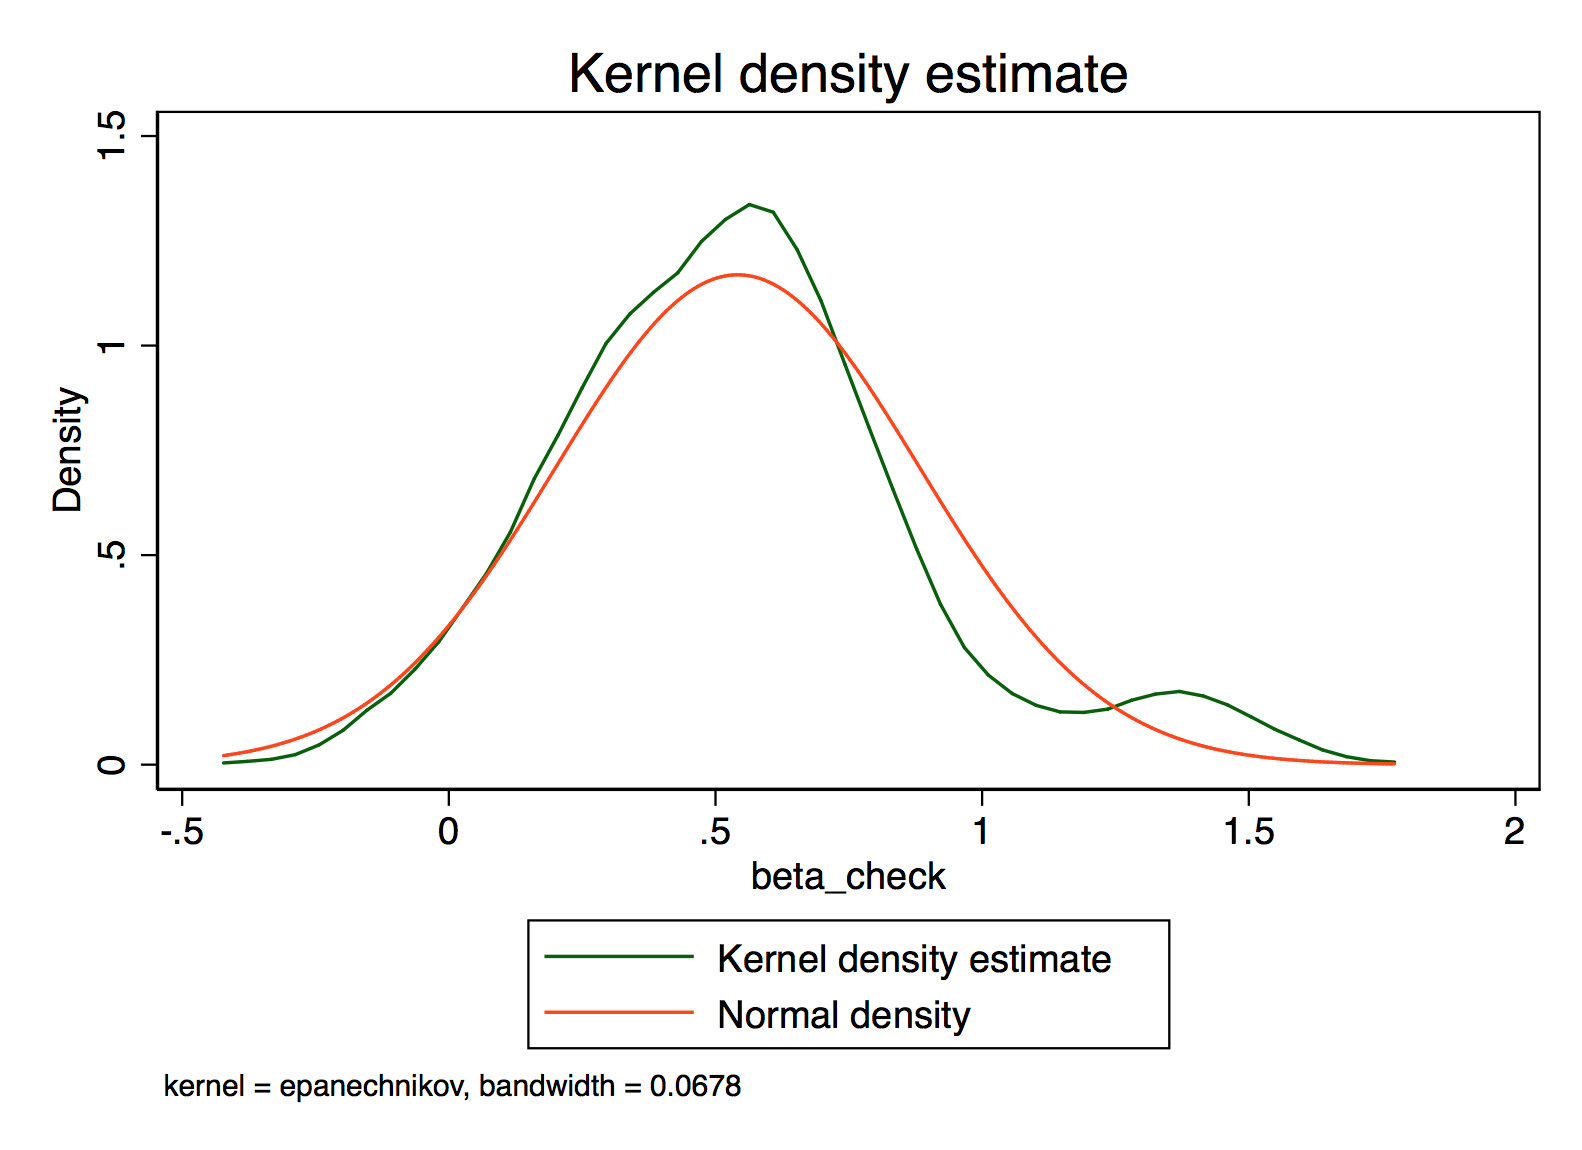
\includegraphics[totalheight=5cm]{hw4_q3_bcheck_stata.png}

Stata Output:
\begin{tabular}{lcccc}
  \hline
&        mean&          sd&         min&         max\\
\hline
$\hat\beta$    &    .5153&    .2900&   -.3544&    1.436\\
$\check\beta$   &    .5415&    .3413&   -.3544&    1.705\\
$\tilde\beta$    &    1.358&    .1663&    .8311&    1.950\\
\hline
\end{tabular}


\subsection{}
Stata Output:

\begin{tabular}{lc}
  \hline
&        Coverage Rate \\
\hline
$\hat\beta$    &    0.201 \\
$\check\beta$   &     0.244 \\
$\tilde\beta$    &   0 \\
\hline
\end{tabular}



\newpage
\section{Code Appendix}
\tiny
\subsection*{Stata}
%\lstinputlisting{hw3.do}
\subsection*{R}
%\lstinputlisting{hw3_q1.R}
%\lstinputlisting{hw3_q2.R}
%\lstinputlisting{hw3_q3.R}
\end{document}
